\chapter{Berechnungen}

\section{$\gamma$- Verfahren}

In der DIN 1052 [] sind zwei unterschiedliche Verfahren angeführt, die für die Schnittgrößenermittlung, nachgiebiger Systeme angewendet werden können:
\\
\begin{itemize}
\item $\gamma$ -Verfahren Abs. 8.6.2 der DIN 1052 []
\item Schubanalogie Anhang D der DIN 1052 []
\end{itemize}
 
In Abbildung \ref{verbunddarstellung} sind die verschiedenen Verbundarten dargestellt. Die Spannungsverteilung ist abhängig vom Verbund der einzelnen Schichten. Bei dem Sandwichaufbau
Holz-Holzspanbeton werden verschiedene Baustoffe verwendet und nachträglich miteinander
verbunden. Zum Einsatz als Verbindungsmittel kommen Kleber und Schrauben.
Daher spielt die Anordnung und Verwendung der Verbindungsmittel eine entscheidende
Rolle über die Aussage des Verbundes. Dies muss bei der statischen Berechnung berücksichtigt
werden. \\
Im [12] sind die Voraussetzungen für eine mathematische korrekte Lösung angeführt. \\

\begin{itemize}
\item statisch bestimmter Einfeldträger
\item sinusförmige Belastung
\item konstante Querschnitte (max. drei Teilquerschnitte)
\item Gültigkeit der Bernoulli-Hypothese in den Teilquerschnitten
\item kontinuierlicher, konstanter Verbund
\item Vernachlässigung der Schubverformung der Teilquerschnitte
\end{itemize}


Für den baupraktisch relevanten Fall der Gleichlast bildet das 
 $\gamma$-Verfahren eine gute
Näherung. Auch Schnitt- und Verformungsgrößen an Durchlaufträgern können ermittelt
werden. Generell berücksichtigt das 
$\gamma$ -Verfahren die Abnahme der Biegesteifigkeit
des Verbundquerschnitts aufgrund der Nachgiebigkeit der Verbundfuge durch den Abminderungsfaktor. Dieser reduziert die Steineranteile der Biegesteifigkeiten der
Teilquerschnitte während die Eigenanteile unverändert bleiben. In der Anwendung für
den Bauteil Holz-Holzspanbeton ist das Verfahren nicht wie in der Literatur dargestellten
Form anzuwenden. Durch die Anwendung des Holzspanbetons als Mittelschicht und dessen Schubweichheit, wird der Träger als 2-teiliger Querschnitt betrachtet. Die Mittelschicht wird als Verbundfuge (Holzleichtbeton) angesehen. Das lässt sich durch den geringen Beitrag der Schicht zur Biegefestigkeit der Gesamtfestigkeit ($E_{HB}\ll E_{C},E_{H}$) und des starren Verbunds zwischen Beton und Holzbeton bzw. Holzbeton und Holz rechtfertigen.



\begin{figure}[h!]
\begin{center}
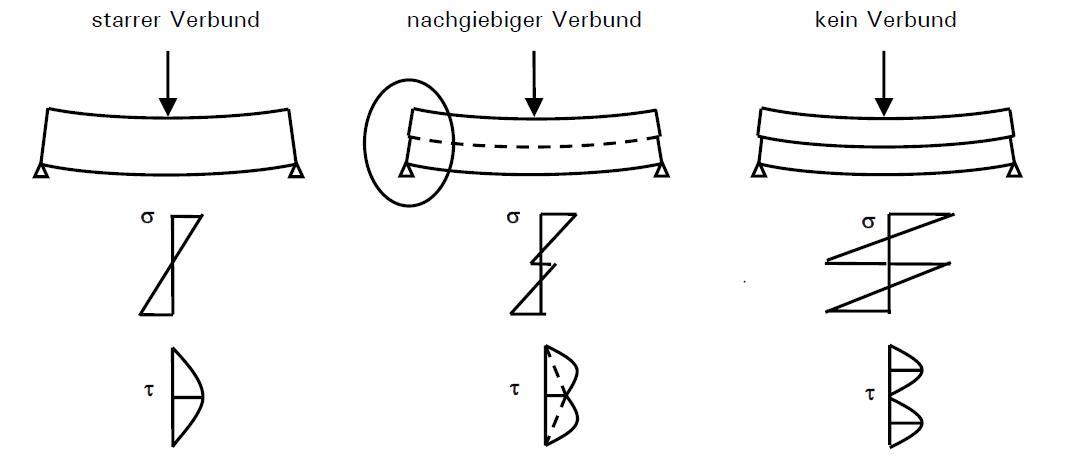
\includegraphics[scale =0.5]{gammaverfahren/abbildungen/verbunddarstellung.jpg}
\caption{Auswirkungen des nachgiebigen Verbundes auf die Spannungsverteilung, []}
\label{verbunddarstellung}
\end{center}
\end{figure}



\begin{figure}[h!]
\begin{center}
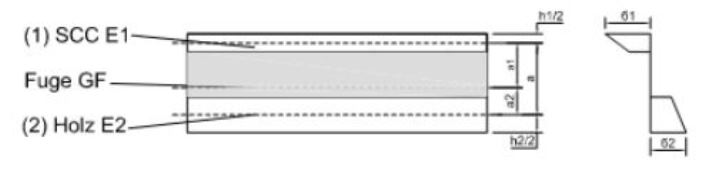
\includegraphics[scale =0.8]{gammaverfahren/abbildungen/verbundquerschnitt.JPG}
\caption{Verbundquerschnitt mit Normalspannungsverlauf im Querschnitt}
\label{verbundquerschnitt}
\end{center}
\end{figure}


\subparagraph{Fugensteifigkeit}
 Die Fugensteifigkeit $c_{F}$ wird analog zu [literatur]als Funktion des Schubmoduls und der
Querschnittsabmessungen angenommen. In der Anwendung des Sandwichbauteils
Holz-Holzspanbeton müssen diese Parameter, und der Einfluss noch experimentell
ermittelt werden.

\begin{equation}
c_{F}=G_{F}\cdot\dfrac{b_{F}}{h_{F}}
\end{equation}

\subparagraph{Nachgiebigkeitsfaktoren} Der Nachgiebigkeitsfaktor 
$\gamma_{1}$ reduziert die Steineranteile des
Teilquerschnitts 1(SCC) und geht in die Berechnung der Spannungsnullebenen und in die
effektive Biegesteifigkeit ein. 

\begin{equation}
\gamma_{1}=\dfrac{1}{1+\dfrac{\Pi^{2}\cdot E_{1}\cdot A_{1}}{c_{F} \cdot l^{2}}};
\gamma_{2}=1,0
\end{equation}

\subparagraph{Lage der ideellen Schwerachsen der Teilquerschnitte}

\begin{equation}
a=\dfrac{h_{1}+h_{2}}{2}+t_{F} \\\\
\end{equation}

\begin{equation}
a_{2}=\dfrac{\gamma_{1} \cdot E_{1} \cdot A_{1} \cdot a_{1}}{\gamma_{1} \cdot E_{1}A_{1} \cdot E_{2}A_{2}}
\end{equation}

\begin{equation}
a_{1}=a-a_{2}
\end{equation}



\subparagraph{effektive Biegefestigkeit}
\begin{equation}
EI_{eff}=E_{1}I_{1}+E_{2}I_{2}+\dfrac{a^{2} \cdot \gamma_{1} \cdot E_{1}A_{1} \cdot E_{2}A_{2}}{\gamma_{1} \cdot E_{1}A_{1} + E_{2}A_{2}}
\end{equation}


\subparagraph{Schnittkräfte:Normalkraft und Biegemoment}
\begin{equation}
M_{i,d}=\dfrac{M_{d}}{EI_{eff}} \cdot E_{i} \cdot I_{i}
\end{equation}


\begin{equation}
N_{i,d}=\dfrac{M_{d}}{EI_{eff}} \cdot \gamma_{1} \cdot a_{i} \cdot E_{i} \cdot A_{i}
\end{equation}

\subparagraph{Normalspannung}

\begin{equation}
\sigma_{i,d}=\dfrac{N_{i,d}}{A_{i}}\pm\dfrac{M_{i,d}}{I_{i}} \cdot \dfrac{h_{i}}{2}
\end{equation}

\subparagraph{Schubspannung}

\begin{equation}
\tau_{i,d}=\dfrac{V_{max}\cdot 0,5 E_{2}\cdot(\dfrac{h_{2}}{2}+a_{2})^2}{EI_{eff}}
\end{equation}


\subparagraph{Berechnung der Durchbiegung für 4-Punkt-Biegeversuch}

\begin{equation}
w_{x}=\dfrac{F \cdot l^{3}}{24 \cdot EI_{eff}}\cdot \dfrac{x}{l} \cdot (3-4\cdot(\dfrac{x}{l})^{2})
\label{math:wx}
\end{equation}

\section{Parameterstudie}
Um die Abhängigkeiten der Eingansparameter darzustellen, wurden die Abbildungen
\ref{c_gamma1} und \ref{gamma1_EIeff.} erstellt. Der entscheidende Eingangsparameter für die Berechnung ist die
Fugensteifigkeit $c_{F}$ . Er besitzt zu Beginn eine sehr hohe Steigung und danach fällt die
Änderung des Wertes 1 nur sehr gering aus. Bei Betrachtung der zweiten Kurve wird
ersichtlich, dass die Steifigkeit in Abhängigkeit von 1 eine fast linearen Zusammenhang
hat. Daher ist Wichtig bei der Betrachtung der Nachrechnung der Fugensteifigkeit
eine erhöhte Aufmerksamkeit zukommen zu lassen.


\begin{figure}[h!]
\begin{center}
\begin{tikzpicture}
\begin{axis}[height=8cm, width=8cm, 
			no markers,xmajorgrids,
			ymajorgrids,xlabel=$c_F$\,$\lbrack MN/m^2 \rbrack $ 											,xmin=0,ymin=0,
			ylabel=$\gamma_{1}$\,$\lbrack 1 \rbrack $]
\addplot table[y=gamma1,x=c]{gammaverfahren/abbildungen/werte.dat};
\end{axis}
\end{tikzpicture}
\caption{Zusammenhang $\gamma$ und $c_{f}$ }
\label{c_gamma1}
\end{center}
\end{figure}


\begin{figure}[h!]
\begin{center}
\begin{tikzpicture}
\begin{axis}[height=8cm, width=8cm, 
			no markers,xmajorgrids,
			ymajorgrids,ylabel=$EI_{eff}$\, $\lbrack MN \cdot m^2 \rbrack $ 											,xmin=0,ymin=0,
			xlabel=$\gamma_{1}$\,$\lbrack 1 \rbrack $]
\addplot table[y=EIeff,x=gamma1]{gammaverfahren/abbildungen/werte.dat};
\end{axis}
\end{tikzpicture}
\caption{Zusammenhang $EI_{eff}$ und$\gamma$ }
\label{gamma1_EIeff}
\end{center}
\end{figure}

\subsection{Nachrechnung der Versuche}

Die Versuche wurden mit dem $\gamma$ -Verfahren nachgerechnet. Es wurde die Durchbiegung
mit der Formel \ref{math:wx} berechnet und an die Versuchskurve angenähert. Die berechnete
Kurve wurde in der Versuchsverlauf so eingebettet, dass sie immer unterhalb (auf
der sicheren Seite) befindet. Im Formelapparat wurde mit dem Wert$ c_{F}$ gearbeitet, um
die Berechnungskurve an die Versuchskurven anzugleichen. Wie in der Parameterstudie
schon beschrieben ist die Fugensteifigkeit cF entscheidend für die Steifigkeit des Systems.
In Abbildungen \ref{V1_kraft_durchbiegung} - \ref{V4_kraft_durchbiegung} sind die Verläufe der einzelnen Versuche abgebildet.
In der Tabelle \ref{tab:Versuchsprogramm} sind die Hauptmerkmale der Versuche und die Ergebnisse der Nachrechnung
aufgelistet.\\

\begin{figure}
\begin{center}

\begin{tikzpicture}
\pgfplotsset{small,width=8cm}
\matrix{
 

\begin{axis}[	title = Bauteilversuch 1,
				legend pos= south east,
				no markers,
				xmajorgrids,ymajorgrids,
				xlabel=Verschiebung\, u \,$\lbrack mm \rbrack $  ,
				ymin=0,xmin=0,
				ylabel=Kraft\, / \,Zylinder\, $\lbrack kN\rbrack $
				]
\addplot table[y=F,x=w1versuch1]{gammaverfahren/abbildungen/versuch1.dat};
\label{pgf:BT1}
\addplot table[y=F,x=w1]{gammaverfahren/abbildungen/versuch1.dat};
\label{pgf:BT1gamma}
\end{axis} 
 
&

\begin{axis}[	title = Bauteilversuch 2,
				legend pos= south east,
				no markers,
				xmajorgrids,ymajorgrids,
				xlabel=Verschiebung\, u \,$\lbrack mm \rbrack $  ,
				ymin=0,xmin=0,
				ylabel=Kraft\, / \,Zylinder\, $\lbrack kN\rbrack $
				]
\addplot table[y=F,x=w1versuch2]{gammaverfahren/abbildungen/versuch2.dat};
\addplot table[y=F,x=w1]{gammaverfahren/abbildungen/versuch2.dat};
\end{axis}

\\

\begin{axis}[	title = Bauteilversuch 3,
				legend pos= south east,
				no markers,
				xmajorgrids,ymajorgrids,
				xlabel=Verschiebung\, u \,$\lbrack mm \rbrack $  ,
				ymin=0,xmin=0,
				ylabel=Kraft\, / \,Zylinder\, $\lbrack kN\rbrack $
				]
\addplot table[y=F,x=w1versuch3]{gammaverfahren/abbildungen/versuch3.dat};
\addplot table[y=F,x=w1]{gammaverfahren/abbildungen/versuch3.dat};
\end{axis}

&

\begin{axis}[	title = Bauteilversuch 4,
				legend pos= south east,
				no markers,
				xmajorgrids,ymajorgrids,
				xlabel=Verschiebung\, u \,$\lbrack mm \rbrack $  ,
				ymin=0,xmin=0,
				ylabel=Kraft\, / \,Zylinder\, $\lbrack kN\rbrack $
				]
\addplot table[green,y=F,x=w1versuch4]{gammaverfahren/abbildungen/versuch4.dat};
\addplot table[y=F,x=w1]{gammaverfahren/abbildungen/versuch4.dat};
\end{axis}

\\
};
\end{tikzpicture}
\fbox{
\ref{pgf:BT1} Versuch \ref{pgf:BT1gamma} Nachrechnung mit $\gamma$-Verfahren
 }
 
\caption{Vergleich der Bauteilversuche mit der Nachrechnung ($\gamma$-Verfahren)}
\label{abb:vergleich_balkendiagramm}
\end{center}
\end{figure}












\begin{table}[h]
\caption{Versuchsprogramm}
\begin{center}
\begin{tabular}{|c|c|c|c|c|c|}
\hline 
\multicolumn{6}{|c|}{ Auswertung der Versuchsergebnisse} \\ 
\hline 
Versuch & $F_{max} $ & Schraubenanzahl/Reihe & $c_{F}$ & $\gamma_{1}$ &$EI_{eff}$ \\ 

 & $[kN]$ & $[1]$ & $[MN/m^{2}]$ & $[1]$ &$[MN*m^{2}$ \\ 
\hline\hline
1 & 74,0 &14& 150 & 0,58 & 13,88 \\ 
\hline 
2  & 30,0 &4& 40 & 0,26 & 8,19 \\ 
\hline 
3 & 58,0 &6& 120 & 0,54 & 13,34 \\ 
\hline 
4  & 7,8 &0& 30,0 & 0,21 &   6,98 \\ 
\hline 
\end{tabular} 
\end{center}
\label{tab:Versuchsprogramm}
\end{table}

\begin{figure}
\begin{center}

\begin{tikzpicture}
\pgfplotsset{small,width=8cm}
\matrix{
 

\begin{axis}[	title = Zusammenhang $EI_{eff}$ und$\gamma$,
				legend pos= south east,
				no markers,
				xmajorgrids,ymajorgrids,
				ymajorgrids,ylabel=$EI_{eff}$\, $\lbrack MN \cdot m^2 \rbrack $ 									,xmin=0,ymin=0,
				xlabel=$\gamma_{1}$\,$\lbrack 1 \rbrack $,
				]
				
\addplot [only marks,color=blue, fill=blue!80!black] coordinates{	(0.58, 13.88)};
\label{pgf:BT1}
\addplot [only marks,color=red, fill=red!80!black] coordinates{	(0.26, 8.19)};
\label{pgf:BT2}
\addplot [only marks,color=brown!60!black, fill=brown!80!black] coordinates{	(0.54, 13.34)};
\label{pgf:BT3}
\addplot [only marks,color=black, fill=black] coordinates{ (0.21,6.98)};
\label{pgf:BT4}
\addplot table[y=EIeff,x=gamma1]{gammaverfahren/abbildungen/werte.dat};				
				
\end{axis} 
 
&

\begin{axis}[	title = Zusammenhang $\gamma$ und $c_{F}$,
				legend pos= south east,
				no markers,
				xmajorgrids,ymajorgrids,
				ymajorgrids,xlabel=$c_F$\,$\lbrack MN/m^2 \rbrack $ 												,xmin=0,ymin=0,
				ylabel=$\gamma_{1}$\,$\lbrack 1 \rbrack $,
				]
\addplot [only marks,color=blue, fill=blue!80!black] coordinates{	(150,0.58)};
\addplot [only marks,color=red, fill=red!80!black] coordinates{	(40, 0.26)};
\addplot [only marks,color=brown!60!black, fill=brown!80!black] coordinates{	(120,0.54)};
\addplot [only marks,color=black, fill=black] coordinates{ (30,0.21)};
\addplot table[y=gamma1,x=c]{gammaverfahren/abbildungen/werte.dat};
\end{axis}


\\
};
\end{tikzpicture}
\fbox{
\ref{pgf:BT1} BT1 \ref{pgf:BT2} BT2  \ref{pgf:BT3} BT3  \ref{pgf:BT4} BT4
 }
 
\caption{Zusammenhänge zwischen $EI_{eff}$ , $\gamma$ und $c_F$)}
\label{abb:zusammmenhaenge}
\end{center}
\end{figure}




\begin{figure}[h!]
\begin{center}
\begin{tikzpicture}
\begin{axis}[height=8cm, width=8cm, 
			no markers,xmajorgrids,
			ymajorgrids,xmajorgrids,
			xlabel=Schraubenanzahl/Reihe ,
			xmin=0,ymin=0,
			ylabel= $c_{F}$\,$\lbrack MN/m^2\rbrack $ ]
\addplot table[y=cF,x=Schraubenanzahl]{gammaverfahren/abbildungen/werte.dat};
\end{axis}
\end{tikzpicture}
\caption{Darstellung der Fugensteifigkeit in Abhängigkeit der Schraubenanzahl}
\label{Fugensteifigkeit-Schraubenanzahl}
\end{center}
\end{figure}




\section{Conclusio:} Wie schon angesprochen wurde die Fugensteifigkeit variiert. In der Abbildung
\ref{Fugensteifigkeit-Schraubenanzahl} ist die Fugensteifigkeit $c_{F}$ in Abhängigkeit der Schraubenanzahl dargestellt.
Es ist ersichtlich, dass der Träger ohne die Verwendung der Schrauben eine geringe
Fugensteifigkeit vorweisen kann. Verwendet man mechanische Verbindungsmitte ist nicht die Anzahl ausschlaggebend, sondern die Anordnung sehr entscheidend. Die Abbildung besitzt einen erheblichen Sprung zwischen 4
und 6 Schrauben und flacht anschließend mit der Zunahme der Schrauben ab.Es muss hier die Anordnung betrachtet werden, denn im Bauteilversuch mit den 4 Schrauben/Reihe sind die Schrauben nicht bis zum Auflager gegangen. Daher ist die Schraubenanzahl und Anordnung ausschlaggebend für das System. Die Erhöhung der
Anzahl der Schrauben wirkt sich nur auf der Seite der Bruchlast aus.Schraubenanzahl
in der Grafik bezieht sich, wie in der Tabelle \ref{tab:Versuchsprogramm} angeführt, auf eine Schraubenreihe.
Anhand der Ergebnisse kann davon aus gegangen werden, dass im Auflagerbereich, sich
ein Zustand einstellt, der mit der Fachwerksanalogie zu vergleichen sein könnte. Die
Schrauben bilden dabei die Zugstäbe ab und das Holzbeton (Velox) die Druckstäbe. Daher ist die
Anwendung von mechanischen Verbindungsmittel unbedingt notwendig, jedoch die Anzahl kann gering gehalten werden. Um
diese Vermutung zu Untermauern, sollten noch einige Verbundversuch durchgeführt werden. Der Aufbau und die Durchführung können im Kapitel 2 nachgelesen werden.
